\documentclass[a4paper,12pt]{report}
\usepackage{graphicx}
\usepackage{listings}

\usepackage{color}
 
\definecolor{codegreen}{rgb}{0,0.6,0}
\definecolor{codegray}{rgb}{0.5,0.5,0.5}
\definecolor{codepurple}{rgb}{0.58,0,0.82}
\definecolor{backcolour}{rgb}{0.95,0.95,0.92}
 
\lstdefinestyle{mystyle}{
    backgroundcolor=\color{backcolour},   
    commentstyle=\color{codegreen},
    keywordstyle=\color{magenta},
    numberstyle=\tiny\color{codegray},
    stringstyle=\color{codepurple},
    basicstyle=\footnotesize,
    breakatwhitespace=false,         
    breaklines=true,                 
    captionpos=b,                    
    keepspaces=true,                 
    numbers=left,                    
    numbersep=5pt,                  
    showspaces=false,                
    showstringspaces=false,
    showtabs=false,                  
    tabsize=2,
    language=python
}
 
\lstset{style=mystyle}

\title{Lanjutan Tugas pemrograman 2 Chapter IV}
\author{Alvian Daniel Sinaga 1184077}
\date{13 November 2019}
\begin{document}
\maketitle
\chapter{CSV dan Pandas}
\section{Teori}
\subsection{CSV}
File Comma Separated Values(CSV) adalah file teks biasa yang berisi daftar data. File-file ini sering digunakan untuk bertukar data antara aplikasi yang berbeda, 
\subsection{Aplikasi pembuat format CSV}
Aplikasi yang dapat membuka dan membuat .Csv yaitu dengan berbagai text-editor seperti Notepad, Wordpad, ataupunMS Excel dengan cara melakukan save as dan simpan sebagai file format csv.
\subsection{Cara Meembuat dan Membaca File CSV di Excel}
\begin{enumerate}
    \item Pertama buka aplikasinya disini saya menggunakan MS Excel
    \item Kemudian isi field yang terdapat pada aplikasi sesuai kebutuhan kita.
    \item kemudian simpan dengan save as 
    \item ketika sudah rubah simpan sebagai ".csv"
    \item lalu simpan , dibawah ini ada conth field yang dibuka, 
    \item dan juga contoh melakukan save as .
    \begin{figure}[!htbp]
\centering
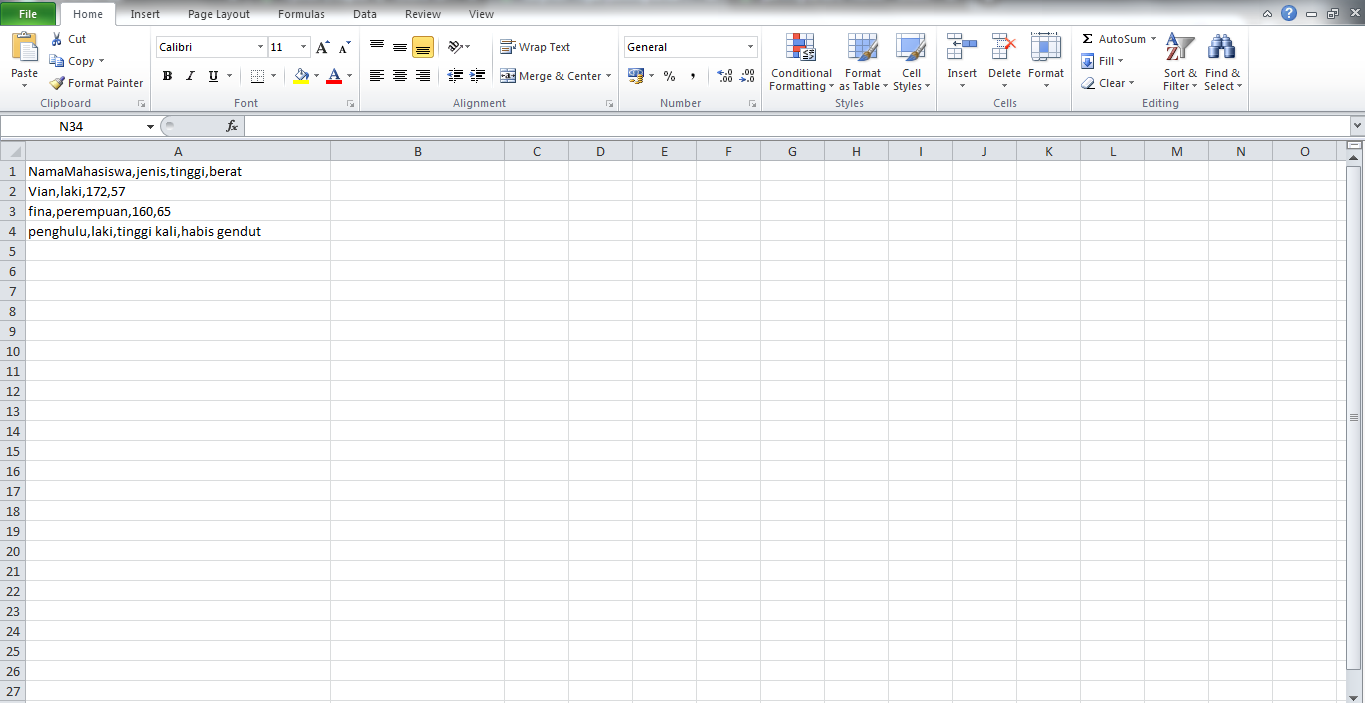
\includegraphics[width=10cm,height=8cm]{figures/1.PNG}
\caption{field Ms.Excel}
\label{penanda}
\end{figure}
    \begin{figure}[!htbp]
\centering
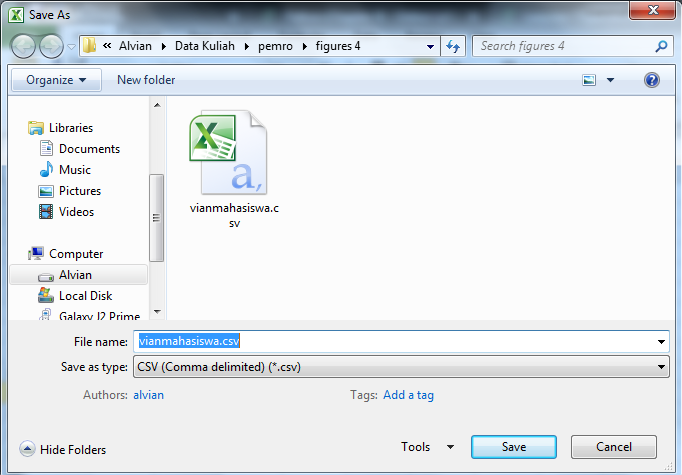
\includegraphics[width=10cm,height=8cm]{figures/2.PNG}
\caption{save format .csv}
\label{penanda}
\end{figure}
    \end{enumerate}
\subsection{CSV Libary}

Manipulasi file csv dengan Python. CSV (Comma Separated Value) merupakan format basis data sederhana dimana setiap record yang ada dipisahkan dengan tanda koma (,) atau titik koma (;). Format data csv ini dapat diolah dengan berbagai text editor dengan mudah.

\subsection{Pandas Libary}
Pandas merupakan sebuah open source python package/library dengan lisensi BSD yang menyediakan banyak perkakas untuk kebutuhan data analisis, manipulasi dan pembersihan data
\subsection{CSV Function}
\begin{enumerate}
    \item writer, untuk menulis atau membuat sebuah file csv dengan record didalamnya.
    \item unregister dialect, untuk menghapus sebuah dialect dari daftar dialect.
    \item get dialect, untuk mengambil data dialect dari daftar dialect.
    \item list dialect, menampilkan semua daftar dialect yang telah didaftarkan.
    \item reader, untuk membaca semua record yang berada didalam file csv.
\end{enumerate}

\subsection{Pandas Function}
\begin{enumerate}
\item pivot table, untuk membuat sebuah spreadsheet dengan style tabel pivot sebagai DataFrame.
\end{enumerate}

\chapter{Keterampilan pemrograman}
\section*{Nomor 1}
\lstinputlisting[language=Python, firstline=3, lastline=8]{src/1184077_csv.py}
\section*{Nomor 2}
\lstinputlisting[language=Python, firstline=10, lastline=14]{src/1184077_csv.py}
\section*{Nomor 3}
\lstinputlisting[language=Python, firstline=3, lastline=9]{src/1184077_pandas.py}
\section*{Nomor 4}
\lstinputlisting[language=Python, firstline=11, lastline=14]{src/1184077_pandas.py}
\section*{Nomor 5}
\lstinputlisting[language=Python, firstline=16, lastline=19]{src/1184077_pandas.py}
\section*{Nomor 6}
\lstinputlisting[language=Python, firstline=21, lastline=26]{src/1184077_pandas.py}
\section*{Nomor 7}
\lstinputlisting[language=Python, firstline=28, lastline=33]{src/1184077_pandas.py}
\section*{Nomor 8}
\lstinputlisting[language=Python, firstline=16, lastline=28]{src/csv_file.py}
\lstinputlisting[language=Python, firstline=1, lastline=4]{src/main.py}
\section*{Nomor 9}
\lstinputlisting[language=Python, firstline=35, lastline=39]{src/1184077_pandas.py}
\lstinputlisting[language=Python, firstline=1, lastline=4]{src/main2.py}



\end{document}